\PassOptionsToPackage{margin=1in}{geometry}
\documentclass[final,3p,times,authoryear]{elsarticle}

\usepackage{amsmath,amssymb,amsfonts,amsthm}
\usepackage{booktabs}
\usepackage{array}
\usepackage{graphicx}
\usepackage{placeins}
\usepackage{algorithm2e}
\usepackage{hyperref}

\newtheorem{assumption}{Assumption}
\newtheorem{lemma}{Lemma}
\newtheorem{proposition}{Proposition}
\newtheorem{corollary}{Corollary}
\newtheorem{theorem}{Theorem}
\newtheorem{remark}{Remark}
\renewcommand{\floatpagefraction}{0.80}

\journal{Transportation Science}

\begin{document}

\begin{frontmatter}

\title{A Two-Phase Integer L-Shaped Method for Stochastic Electric-Bus Wireless Charging Infrastructure Planning}

\author[inst1]{Author Name}
\address[inst1]{Affiliation}

\begin{abstract}
This abstract will be written after the main body is stable.
\end{abstract}

\begin{keyword}
Wireless charging \sep electric bus \sep stochastic programming \sep integer L-shaped method \sep Benders decomposition
\end{keyword}

\end{frontmatter}

\section{Introduction}
\label{sec:introduction}

Electrifying bus fleets requires coordinated decisions on charging infrastructure, battery capacity, and daily charging operations.
Wireless charging technologies expand the set of feasible charging opportunities by allowing buses to charge at selected stops or road links during regular service.
This creates a planning trade-off: more in-route wireless charging can reduce battery requirements and residual plug-in fast-charging needs, but installing such infrastructure is costly and must be robust to future service plans.

The planning difficulty is amplified by service-plan uncertainty.
Transit agencies may adjust routes, timetables, and duty assignments over a medium-term planning horizon, while embedded wireless facilities are shared physical investments that cannot be changed after the scenario is realized.
Thus, a first-stage wireless charging layout must support multiple possible representative operating days.

Wireless infrastructure also changes downstream operational coupling.
After a service-plan scenario is realized, the operator chooses route-level battery capacities and charging schedules.
SWC and DWC opportunities affect how much energy can be obtained during service, which in turn changes battery sizing and the residual demand for existing plug-in fast chargers.
Because plug-in fast chargers are limited shared operational resources, residual fast-charging demand couples otherwise route-level recourse decisions.

These features lead to a two-stage stochastic mixed-integer planning problem.
The first stage selects shared wireless charging facilities, and the second stage contains scenario-dependent battery and charging-operation decisions.
The recourse problem has discrete battery choices, operational charging decisions, and shared plug-in fast-charger capacity constraints, making the deterministic equivalent and a direct integer L-shaped decomposition computationally challenging.

This paper develops an exact reformulation-enabled integer L-shaped method for this problem class.
The three algorithmic contributions are nested rather than independent.
First, we introduce an exact structure-exposing lifted reformulation that places scenario-dependent battery configuration variables in the master while preserving their scenario-adaptive role.
Second, we use the lifted structure to build a nested scenario--route relaxation--verification decomposition: Phase 1 relaxes shared plug-in fast-charger capacity coupling and operational integrality to obtain route-level LP lower bounds, and Phase 2 restores the exact scenario-level mixed-integer operational recourse.
Third, we derive joint-resource direction-selective monotonicity cuts that exploit the partial order induced by wireless facility additions and battery-capacity upgrades.
The dependency chain is lifting, route-decomposable relaxation, exposed joint-resource order, and strengthened cuts.

The computational study uses Tower-derived electric-bus planning instances as a realistic test bed for the algorithm.
The experiments first give a compact planning interpretation, then evaluate the algorithm through network-scale ablation, scenario-count scalability, and capacity-coupling stress tests.
The evidence is intended to show which components are necessary for scalability and how the method behaves when the Phase 1 relaxation becomes more or less aligned with the exact Phase 2 feasible region.

\section{Literature Review}
\label{sec:literature}

This section reviews two streams of literature that define the paper's application structure and algorithmic positioning.
The first stream is electric-bus charging and wireless infrastructure planning, which motivates the interaction among wireless facilities, battery choices, and existing plug-in fast-charging resources.
The second stream is stochastic facility-location modeling and decomposition, which provides the methodological context for two-stage mixed-integer planning with scenario-dependent recourse.
The review is organized to keep the transportation discussion concise and to focus on the shared-resource mixed-integer recourse structure used by the proposed algorithm.

\subsection{Electric-bus charging and wireless infrastructure planning}
\label{subsec:lit-wireless-bus}

% TODO: Add verified citations for SWC/DWC planning, electric-bus battery sizing, plug-in charging scheduling, and route-level energy management.

Electric-bus charging studies commonly coordinate infrastructure deployment, battery sizing, vehicle or charging schedules, and service feasibility.
These decisions are often formulated as integrated optimization models because charging resources, route energy requirements, and schedule feasibility interact.
Depot and plug-in fast-charging studies emphasize charger availability and charging schedules, whereas opportunity-charging studies add charging possibilities during service.

Wireless charging infrastructure planning extends this setting by considering stationary wireless charging at stops and dynamic wireless charging on road links.
This literature provides modeling elements that are central to our application: candidate wireless facilities, route-level energy feasibility, battery-capacity implications, and charging-operation constraints.
It also motivates the coexistence of wireless facilities with existing plug-in fast-charging resources.

Our use of this stream is structural.
We adopt wireless-facility placement, route-level battery choices, representative-day charging operations, and existing plug-in fast chargers as the application objects of the model.
We do not focus on real-time charging control, bus dispatch, or traffic operations; instead, these objects define a long-term planning setting whose shared-resource mixed-integer recourse structure is reviewed methodologically next.

\subsection{Stochastic facility-location models and decomposition methods}
\label{subsec:lit-stochastic-decomposition}

% TODO: Add verified citations for stochastic facility location and stochastic network design.
% TODO: Add verified citations for integer L-shaped methods and mixed-integer recourse.
% TODO: Add verified citations for partial Benders or lifted master reformulations.
% TODO: Add verified citations for relaxation-based recourse switching and Benders subproblem decomposition.
% TODO: Add verified citations for logic-based, combinatorial, and monotonicity-based Benders cuts.

Stochastic facility-location and network-design models provide the optimization background for here-and-now infrastructure decisions under uncertain future conditions.
In these models, scenarios typically represent uncertain demand, service requirements, or operating conditions, and the recourse problem evaluates the consequence of a first-stage design after a scenario is realized.
Benders decomposition, integer L-shaped methods, and logic-based Benders decomposition provide the standard decomposition language for such two-stage models, especially when the deterministic equivalent is too large or the recourse problem contains discrete decisions.

Within this decomposition family, computational performance is shaped by two broad design dimensions.
The first is the decomposition or reformulation choice: what information is retained in the master problem, what remains in the scenario subproblems, and whether the subproblems can be decomposed or relaxed without losing useful bound information.
The second is the separation strategy: how feasibility and optimality information from the subproblems is converted into cuts, and whether those cuts exploit problem-specific structure beyond a basic no-good exclusion.

Research on decomposition for mixed-integer recourse has developed techniques along both dimensions.
On the reformulation side, stronger master representations, partial recourse descriptions, relaxed subproblems, and internal subproblem decompositions can improve lower bounds or reduce separation cost.
On the cut side, integer L-shaped cuts, logic-based Benders cuts, combinatorial cuts, valid inequalities, and dominance-based cuts can exploit structure that is not captured by generic linear duality.
The effectiveness and validity of these enhancements are structure dependent, which is why successful decomposition algorithms are often tailored to the recourse model rather than transferred directly from one application to another.

This paper follows that tailored-decomposition perspective.
The electric-bus wireless-charging setting creates a shared-resource mixed-integer recourse structure with scenario-dependent battery choices, route-level operating decisions, and plug-in fast-charger capacity coupling.
The proposed method instantiates the two design dimensions above through a reformulation-enabled integer L-shaped algorithm: it changes the master--subproblem organization, uses a relaxation--verification separation scheme, and derives cuts from the joint facility--battery structure while retaining exact recourse verification.

\section{Problem Formulation and Recourse Structure}
\label{sec:model}

This section formulates the wireless charging infrastructure planning problem as a two-stage stochastic program.
The formulation separates long-lived wireless-facility decisions from scenario-adaptive battery and charging decisions, and then identifies the recourse structure used by the algorithm in Section~\ref{sec:method}.

\subsection{Two-stage stochastic formulation}
\label{subsec:two-stage-formulation}

Let $\Omega$ be the set of service-plan scenarios, and let $p_\omega$ be the probability of scenario $\omega \in \Omega$, where $p_\omega>0$ and $\sum_{\omega\in\Omega}p_\omega=1$.
Each scenario represents one plausible future service plan and fixes the route frequencies, timetables, bus trip chains, active-fleet requirements, and trip-level energy requirements, while the operated route set $\mathcal{R}$ is common across scenarios.
The planner first installs long-lived wireless charging facilities before the future service plan is known.
After a scenario is realized, the second-stage recourse selects route-level battery capacities and the corresponding representative-day charging allocation and energy-management decisions.

Let $\mathcal{S}$ be the station set, $\mathcal{L}$ the directed link set between consecutive stations, and $\mathcal{C}\subseteq\mathcal{S}$ the set of existing interchanges or hubs equipped with plug-in chargers.
Stationary wireless charging (SWC) can be installed at any station in $\mathcal{S}\setminus\mathcal{C}$, while dynamic wireless charging (DWC) can be installed on any directed link in $\mathcal{L}$.
The first-stage binary variables $w_s^{\mathrm{S}}$ and $w_l^{\mathrm{D}}$ indicate whether SWC is installed at station $s\in\mathcal{S}\setminus\mathcal{C}$ and DWC is installed on link $l\in\mathcal{L}$, respectively.
Existing plug-in chargers at stations in $\mathcal{C}$ are pre-existing resources with limited shared capacity and are not candidates for SWC deployment.

The compact two-stage stochastic formulation is
\begin{align}
    \min_{w^{\mathrm{S}},w^{\mathrm{D}}} \quad
        & C^{\mathrm{fac}}(w)
        +
        \sum_{\omega \in \Omega} p_\omega \Phi_\omega(w)
        \label{eq:two-stage-model} \\
    \mathrm{s.t.} \quad
        & w_s^{\mathrm{S}} \in \{0,1\},
        && s \in \mathcal{S}\setminus\mathcal{C},
        \label{eq:swc-domain} \\
        & w_l^{\mathrm{D}} \in \{0,1\},
        && l \in \mathcal{L}.
        \label{eq:dwc-domain}
\end{align}
where $w=(w^{\mathrm{S}},w^{\mathrm{D}})$ and
\[
    C^{\mathrm{fac}}(w)=\sum_{s \in \mathcal{S}\setminus\mathcal{C}} c_s^{\mathrm{S}} w_s^{\mathrm{S}}+\sum_{l \in \mathcal{L}} c_l^{\mathrm{D}} w_l^{\mathrm{D}}.
\]
Here $c_s^{\mathrm{S}}$ and $c_l^{\mathrm{D}}$ are the representative-day equivalent costs of installing SWC at station $s$ and DWC on link $l$, respectively.
Facility and battery investment costs are converted to representative-day equivalents to match the charging-cost scale.
The vector $w$ is the nonanticipative here-and-now facility decision, and $\Phi_\omega(w)$ is the optimal second-stage value in scenario $\omega$.

The scenario decisions consist of route-level battery selection variables $z_{\omega,r,k}$, plug-in charger occupancy variables collected in $x_\omega$, and remaining operating variables collected in $y_\omega$, including charging amounts and battery energy states.
For a fixed facility layout $w$, the scenario recourse value $\Phi_\omega(w)$ is the minimum scenario cost
\begin{equation}
    \Phi_\omega(w)
    =
    \min_{z_\omega,x_\omega,y_\omega}
    \left\{
        C^{\mathrm{bat}}_\omega(z_\omega) + C^{\mathrm{chg}}_\omega(y_\omega):
        (z_\omega,x_\omega,y_\omega)\in\mathcal{X}_\omega(w)
    \right\}.
    \label{eq:recourse-value}
\end{equation}
The next subsection expands $\mathcal{X}_\omega(w)$.

\subsection{Scenario recourse formulation}
\label{subsec:scenario-recourse-formulation}

For a fixed scenario $\omega$, the recourse formulation uses route-indexed trip-chain data.
For each route $r\in\mathcal R$, $\mathcal{M}_{\omega,r}$ is the set of trip chains, $\mathcal{A}_{\omega,r}$ is the set of directed traversals, and $\mathcal{V}^{\mathrm{P}}_{\omega,r}$ and $\mathcal{V}^{\mathrm{S}}_{\omega,r}$ are the plug-in and SWC station visits.
Each trip chain corresponds to one bus, so $n_{\omega,r}=|\mathcal{M}_{\omega,r}|$ is the route fleet size in scenario $\omega$.
A consolidated notation table is provided in Appendix~\ref{app:model-details}.

\paragraph{Recourse costs.}
Battery options $\mathcal{K}$ have capacities $\beta_k$, with representative-day equivalent unit cost $c^{\mathrm{bat}}$.
Operating cost is based on grid-side energy purchased through plug-in charging, stationary wireless charging, dynamic wireless charging, and overnight depot charging.
The corresponding charging amounts are $q_v^{\mathrm{P}}$, $q_v^{\mathrm{S}}$, $q_a^{\mathrm{D}}$, and $q_m^{\mathrm{N}}$, with nonnegative daytime and overnight electricity prices $c^{\mathrm{day}}$ and $c^{\mathrm{night}}$.
The scenario battery cost is
\[
    C^{\mathrm{bat}}_\omega(z_\omega)
    =
    c^{\mathrm{bat}}
    \sum_{r \in \mathcal{R}}
    n_{\omega,r}
    \sum_{k \in \mathcal{K}}
    \beta_k z_{\omega,r,k}.
\]
The scenario charging cost is
\[
    C^{\mathrm{chg}}_\omega(y_\omega)
    =
    c^{\mathrm{day}}
    \left(
    \sum_{r \in \mathcal{R}}
    \sum_{v \in \mathcal{V}^{\mathrm{P}}_{\omega,r}} q_v^{\mathrm{P}}
    +
    \sum_{r \in \mathcal{R}}
    \sum_{v \in \mathcal{V}^{\mathrm{S}}_{\omega,r}} q_v^{\mathrm{S}}
    +
    \sum_{r \in \mathcal{R}}
    \sum_{a \in \mathcal{A}_{\omega,r}} q_a^{\mathrm{D}}
    \right)
    +
    c^{\mathrm{night}}
    \sum_{r \in \mathcal{R}}
    \sum_{m \in \mathcal{M}_{\omega,r}}
    q_m^{\mathrm{N}}.
\]

\paragraph{Battery configuration.}
The route-level battery-choice constraints are
\begin{align}
    & \sum_{k \in \mathcal{K}} z_{\omega,r,k} = 1,
    && r \in \mathcal{R},
    \label{eq:one-battery} \\
    & B_{\omega,r}
    =
    \sum_{k \in \mathcal{K}} \beta_k z_{\omega,r,k},
    && r \in \mathcal{R},
    \label{eq:battery-size} \\
    & z_{\omega,r,k} \in \{0,1\},
    && r \in \mathcal{R},\ k \in \mathcal{K}.
    \label{eq:z-domain}
\end{align}
Constraints~\eqref{eq:one-battery}--\eqref{eq:z-domain} select one common battery option for all buses assigned to each route and define the induced route battery capacity $B_{\omega,r}$.

\paragraph{Shared plug-in charging.}
Plug-in charger use is modeled over scenario time slots $\mathcal{T}_\omega$.
A visit $v$ can use plug-in charging only during $\mathcal{T}_v\subseteq\mathcal{T}_\omega$, and $s(v)$ maps the visit to its station.
The binary variable $x_{v\tau}$ records whether visit $v$ occupies a plug-in charger in time slot $\tau$; each occupied slot delivers up to $\kappa$ units of grid-side energy, and station $s$ has capacity $U_s$.
The plug-in charging constraints are
\begin{align}
    & 0
    \leq
    q_v^{\mathrm{P}}
    \leq
    \kappa
    \sum_{\tau \in \mathcal{T}_v} x_{v\tau},
    && r \in \mathcal{R},\ v \in \mathcal{V}^{\mathrm{P}}_{\omega,r},
    \label{eq:plugin-charge-limit} \\
    & \sum_{r \in \mathcal{R}}
    \sum_{\substack{v \in \mathcal{V}^{\mathrm{P}}_{\omega,r}:\\ s(v)=s,\ \tau\in\mathcal{T}_v}}
    x_{v\tau}
    \leq
    U_s,
    && s \in \mathcal{C},\ \tau \in \mathcal{T}_\omega,
    \label{eq:plugin-capacity} \\
    & x_{v\tau} \in \{0,1\},
    && r \in \mathcal{R},\ v \in \mathcal{V}^{\mathrm{P}}_{\omega,r},\ \tau \in \mathcal{T}_v.
    \label{eq:x-domain}
\end{align}
Constraints~\eqref{eq:plugin-charge-limit}--\eqref{eq:x-domain} define plug-in charging amounts, plug-in charger occupancy, and station-time capacity.
The shared plug-in charger-capacity constraint~\eqref{eq:plugin-capacity} provides the main cross-route coupling within a scenario.

\paragraph{Route-local operational feasibility.}
Route energy feasibility is written over station visits $\mathcal{V}_{\omega,r}$ and directed traversals $\mathcal{A}_{\omega,r}$.
The mappings $\ell(a)$, $\mathrm{tail}(a)$, and $\mathrm{head}(a)$ connect each traversal to its physical link and adjacent visits.
Traversal and depot energy requirements are represented by $d_a$, $d_m^0$, and $d_m^N$, while $\bar q$ and $\eta$ collect charging-opportunity limits and charging efficiencies.
The variables $e_v^{\mathrm{arr}}$ and $e_v^{\mathrm{dep}}$ are the battery energy states at arrival and departure of visit $v$.
The state-of-charge fractions are bounded by $\underline{\rho}$ and $\overline{\rho}$, and $v_m^0$ and $v_m^N$ denote the first and last visits of trip chain $m$; detailed notation is listed in Appendix~\ref{app:model-details}.
Trip-level energy requirements are exogenous and do not vary with the selected battery capacity.
Overnight depot charging is assumed to have sufficient power and capacity to restore all buses to the prescribed initial state of charge before the next representative day.
Event-level variables suppress scenario and route indices because each visit and traversal is already a scenario-route-specific copy.
Charging quantities are nonnegative continuous grid-side energy variables, and battery-energy states are continuous.
For each route $r\in\mathcal R$, the route-local operational constraints are
\begin{align}
    & 0
    \leq
    q_v^{\mathrm{S}}
    \leq
    \bar{q}^{\mathrm{S}}_v w_{s(v)}^{\mathrm{S}},
    && v \in \mathcal{V}^{\mathrm{S}}_{\omega,r},
    \label{eq:swc-charge-limit} \\
    & 0
    \leq
    q_a^{\mathrm{D}}
    \leq
    \bar{q}^{\mathrm{D}}_a w_{\ell(a)}^{\mathrm{D}},
    && a \in \mathcal{A}_{\omega,r}.
    \label{eq:dwc-charge-limit} \\
    & \underline{\rho} B_{\omega,r}
    \leq
    e^{\mathrm{arr}}_v
    \leq
    \overline{\rho} B_{\omega,r},
    && v \in \mathcal{V}_{\omega,r},
    \label{eq:soc-arr-bound} \\
    & \underline{\rho} B_{\omega,r}
    \leq
    e^{\mathrm{dep}}_v
    \leq
    \overline{\rho} B_{\omega,r},
    && v \in \mathcal{V}_{\omega,r},
    \label{eq:soc-dep-bound} \\
    & e^{\mathrm{dep}}_v
    =
    e^{\mathrm{arr}}_v
    +
    \eta^{\mathrm{P}}
    q_v^{\mathrm{P}},
    && v \in \mathcal{V}^{\mathrm{P}}_{\omega,r},
    \label{eq:station-energy-balance} \\
    & e^{\mathrm{dep}}_v
    =
    e^{\mathrm{arr}}_v
    +
    \eta^{\mathrm{S}}
    q_v^{\mathrm{S}},
    && v \in \mathcal{V}^{\mathrm{S}}_{\omega,r}, \notag \\
    & e^{\mathrm{arr}}_{\mathrm{head}(a)}
    =
    e^{\mathrm{dep}}_{\mathrm{tail}(a)}
    -
    d_a
    +
    \eta^{\mathrm{D}}
    q_a^{\mathrm{D}},
    && a \in \mathcal{A}_{\omega,r},
    \label{eq:link-energy-balance} \\
    & e^{\mathrm{arr}}_{v_m^{0}}
    =
    \overline{\rho} B_{\omega,r}
    -
    d_m^{0},
    && m \in \mathcal{M}_{\omega,r},
    \label{eq:initial-boundary-energy} \\
    & e^{\mathrm{dep}}_{v_m^{N}}
    -
    d_m^{N}
    \geq
    \underline{\rho} B_{\omega,r},
    && m \in \mathcal{M}_{\omega,r},
    \label{eq:return-boundary-energy} \\
    & \eta^{\mathrm{P}} q_m^{\mathrm{N}}
    =
    \overline{\rho} B_{\omega,r}
    -
    e^{\mathrm{dep}}_{v_m^{N}}
    +
    d_m^{N},
    && m \in \mathcal{M}_{\omega,r}.
    \label{eq:overnight-charge-balance}
\end{align}
Constraints~\eqref{eq:swc-charge-limit}--\eqref{eq:dwc-charge-limit} link route operations to first-stage wireless-facility decisions, and constraints~\eqref{eq:soc-arr-bound}--\eqref{eq:soc-dep-bound} impose arrival and departure state-of-charge bounds.
Constraints~\eqref{eq:station-energy-balance}--\eqref{eq:link-energy-balance} update the energy state through station charging and directed traversals, while constraints~\eqref{eq:initial-boundary-energy}--\eqref{eq:overnight-charge-balance} close each trip chain through depot movements and overnight recharge.

\subsection{Recourse structure}
\label{subsec:recourse-structure}

For a fixed facility layout $w$, the expected recourse term is separable across scenarios. This yields a standard integer L-shaped reference in which each scenario is evaluated as a monolithic mixed-integer recourse problem over $(z_\omega,x_\omega,y_\omega)$. We refer to this direct decomposition as Natural ILS.
The recourse problem also exhibits conditional route locality. Constraints~\eqref{eq:swc-charge-limit}--\eqref{eq:overnight-charge-balance} are imposed independently by route, whereas the shared plug-in charger-capacity constraint~\eqref{eq:plugin-capacity} couples plug-in occupancy across routes at each station--time pair.
Finally, the formulation induces a facility--battery resource order. Under the model specification that trip-level energy consumption is independent of the selected battery capacity, additional wireless facilities and larger route batteries preserve operational feasibility under resource-dominating configurations and cannot increase the minimum charging cost.

These properties define a layered recourse structure comprising scenario-dependent discrete battery configurations, conditionally route-local operations, and limited shared-capacity coupling. Section~\ref{sec:method} develops an exact decomposition method tailored to this structure.

\section{Reformulation-Enabled Integer L-Shaped Method}
\label{sec:method}

This section develops the proposed method, starting from the lifted reformulation rather than from the natural decomposition baseline.
The method has three linked components: an exact structure-exposing lifted reformulation, a nested scenario--route relaxation--verification decomposition, and joint-resource direction-selective monotonicity cuts.
The notation in this section separates master decisions from scenario operating evaluations.
Let $\mathcal{Q}_\omega(w,z_\omega)$ denote the exact operational feasible set after the battery configuration is fixed, and let $Q_\omega(w,z_\omega)$ denote the corresponding exact operational recourse value.
Let $\mathcal{Q}^R_\omega(w,z_\omega)$ and $Q^R_\omega(w,z_\omega)$ denote the Phase 1 relaxation.
The variable $\theta_\omega$ is the master approximation of $Q_\omega(w,z_\omega)$, and $\mathcal{L}_\omega$ is the current set of valid lower-bounding cuts for scenario $\omega$.

\subsection{Lifted master reformulation}
\label{subsec:lifted-reformulation}

The natural integer L-shaped formulation in Section~\ref{sec:model} keeps only the facility vector $w$ in the master and evaluates each scenario through the battery-and-operation recourse value $\Phi_\omega(w)$.
The lifted reformulation moves the scenario-level battery variables $z_\omega$ into the master so that the master decides the facility layout and the battery configuration together.

For fixed $(w,z_\omega)$, the exact operational recourse value is
\begin{equation}
    Q_\omega(w,z_\omega)
    =
    \min_{y_\omega}
    \left\{
    C^{\mathrm{op}}_\omega(y_\omega)
    :
    y_\omega \in \mathcal{Q}_\omega(w,z_\omega)
    \right\}.
    \label{eq:operational-recourse}
\end{equation}
The scenario value from Section~\ref{sec:model} can then be written as
\begin{equation}
    \Phi_\omega(w)
    =
    \min_{z_\omega}
    \left\{
    C^{\mathrm{bat}}_\omega(z_\omega)
    +
    Q_\omega(w,z_\omega)
    :
    z_\omega \in \mathcal{Z}_\omega
    \right\}.
    \label{eq:lifted-scenario-value}
\end{equation}

The lifted master is
\begin{align}
    \min_{w,z,\theta} \quad
        & C^{\mathrm{fac}}(w)
        + \sum_{\omega \in \Omega} p_\omega
        \left[
            C^{\mathrm{bat}}_\omega(z_\omega) + \theta_\omega
        \right]
        \label{eq:master-obj} \\
    \mathrm{s.t.} \quad
        & z_\omega \in \mathcal{Z}_\omega,
        && \omega \in \Omega,
        \label{eq:master-z-domain} \\
        & \theta_\omega \geq \ell, && \omega \in \Omega,\ \ell \in \mathcal{L}_\omega,
        \label{eq:benders-cuts} \\
        & w_j \in \{0,1\},
        && j \in \mathcal{J},
        \label{eq:master-w-domain} \\
        & z_{\omega r k} \in \{0,1\},
        && \omega \in \Omega,\ r \in \mathcal{R}_\omega,\ k \in \mathcal{K}_r.
        \label{eq:binary-decisions}
\end{align}
Here $\mathcal{Z}_\omega$ is the battery-choice feasible set from Section~\ref{sec:model}.

\begin{proposition}[Exactness of the lifted master reformulation]
\label{prop:equivalence}
The lifted master reformulation is equivalent to the natural integer L-shaped formulation in Section~\ref{sec:model}.
\end{proposition}

\begin{proof}[Proof sketch]
For any feasible solution of the natural formulation, the same $(w,z_\omega)$ pair is feasible in the lifted master, and the exact operational value $Q_\omega(w,z_\omega)$ is unchanged.
Conversely, every feasible lifted solution induces the same $(w,z_\omega)$ configuration and the same objective value in the natural formulation because $z_\omega$ remains scenario dependent and has no cross-scenario nonanticipativity.
\qedhere
\end{proof}

This reformulation only changes the layer at which $z_\omega$ is optimized.
It does not impose cross-scenario nonanticipativity on $z_\omega$ and does not claim novelty from moving recourse variables in general.
Its role is to isolate the remaining operational recourse and expose the facility--battery resource structure used by the Phase 1 decomposition and monotonicity cuts.

\subsection{Two-phase lower bounding and exact verification}
\label{subsec:two-phase-framework}

Given $(w,z_\omega)$, the exact operational subproblem remains difficult because it still contains shared plug-in fast-charger capacity constraints and binary operational decisions.
The two-phase scheme separates lower-bound generation from exact verification.

\subsubsection{Phase 1: route-level LP relaxation}
\label{subsec:phase-one}

Phase 1 relaxes shared plug-in fast-charger capacity coupling and operational integrality in the exact operational subproblem.
As a result, the remaining model decomposes by route and yields smaller LP subproblems whose dual solutions generate lower-bound cuts.
The closer the Phase 1 relaxation is to the Phase 2 feasible region, the tighter these lower bounds can be.
This Phase 1--Phase 2 gap is driven by how binding the relaxed constraints are; in the wireless charging application, the key relaxed coupling is the capacity of existing plug-in fast chargers that serve residual fast-charging demand after wireless charging opportunities and battery choices are fixed.

\begin{proposition}[Phase 1 relaxation and decomposition]
\label{prop:phase-one-lb}
For any fixed master solution $(w,z_\omega)$, the Phase 1 relaxation satisfies
\begin{equation}
    Q^R_\omega(w,z_\omega) \leq Q_\omega(w,z_\omega).
    \label{eq:phase-one-lb}
\end{equation}
Moreover, the Phase 1 relaxation decomposes exactly into independent route-level LP subproblems:
\begin{equation}
    Q^R_\omega(w,z_\omega)
    =
    \sum_{r \in \mathcal{R}_\omega} Q^R_{\omega r}(w,z_{\omega r}).
    \label{eq:phase-one-decomposition}
\end{equation}
\end{proposition}

\begin{proof}[Proof sketch]
Phase 1 removes constraints and integrality requirements from the exact operational subproblem, so its feasible region contains the exact feasible region and its minimization value is no larger.
After the shared plug-in fast-charger capacity coupling is relaxed, the remaining route-specific constraints and objective terms separate by route, which gives the additive decomposition.
\qedhere
\end{proof}

Any LP-dual lower-bounding cut generated from Phase 1 is therefore valid for the exact operational value.
For a violated route-level LP relaxation, a representative cut can be written as
\begin{equation}
    \theta_\omega
    \geq
    \alpha_\omega
    + \sum_{j \in \mathcal{J}} \pi_{\omega j} w_j
    + \sum_{r \in \mathcal{R}_\omega}
      \sum_{k \in \mathcal{K}_r}
      \lambda_{\omega r k} z_{\omega r k},
    \label{eq:phase-one-dual-cut}
\end{equation}
where the coefficients are obtained from the Phase 1 LP dual.

\subsubsection{Phase 2: mixed-integer verification}
\label{subsec:phase-two}

Phase 2 restores the exact operational MIP for fixed $(w,z_\omega)$.
It produces exact feasibility judgments, exact operational costs, and incumbent upper bounds:
\begin{equation}
    UB =
    C^{\mathrm{fac}}(w)
    + \sum_{\omega \in \Omega} p_\omega
    \left[
        C^{\mathrm{bat}}_\omega(z_\omega)
        + Q_\omega(w,z_\omega)
    \right].
    \label{eq:upper-bound}
\end{equation}
Because Phase 2 evaluates the same exact operational subproblem that appears in the lifted formulation, it preserves the exactness of the model.

\subsection{Monotonicity-based strengthened cuts}
\label{subsec:strengthened-cuts}

The full method strengthens both the relaxed and exact separation loops whenever the corresponding monotonicity-based cut is valid for the exact recourse function.
The key structure is the joint partial order induced by wireless facility additions and route-level battery-capacity upgrades.

\begin{assumption}[Monotone feasibility and operating cost]
\label{ass:monotonicity}
For a fixed service-plan scenario, opening additional wireless facilities or selecting weakly larger battery capacities cannot remove any operational schedule that was previously feasible.
Moreover, these changes cannot increase the optimal operational recourse value $Q_\omega(w,z_\omega)$.
\end{assumption}

Assume that the battery options for each route are indexed in nondecreasing capacity order.
Consider a Phase 2 solution $(w^*,z^*_\omega)$ for scenario $\omega$, and let $k^*_{\omega r}$ be the selected battery-capacity option for route $r$ in this solution.
Define
\begin{equation}
    I_\omega(w,z_\omega;w^*,z^*_\omega)
    =
    \sum_{j: w^*_j=0} w_j
    +
    \sum_{r \in \mathcal{R}_\omega}
    \sum_{k \in \mathcal{K}_r: k > k^*_{\omega r}}
    z_{\omega r k}.
    \label{eq:monotone-indicator}
\end{equation}
The indicator is zero when a candidate opens no additional facility and upgrades no route battery relative to $(w^*,z^*_\omega)$.

\begin{proposition}[Strengthened feasibility cut]
\label{prop:strengthened-feasibility}
Suppose Assumption~\ref{ass:monotonicity} holds and the Phase 2 operational subproblem for scenario $\omega$ is infeasible at $(w^*,z^*_\omega)$.
Then
\begin{equation}
    I_\omega(w,z_\omega;w^*,z^*_\omega) \geq 1
    \label{eq:strengthened-feasibility-cut}
\end{equation}
is a valid feasibility cut.
\end{proposition}

\begin{proof}[Proof sketch]
Any solution with zero indicator is dominated by the infeasible configuration and cannot restore feasibility by monotonicity.
\qedhere
\end{proof}

\begin{proposition}[Strengthened optimality cut]
\label{prop:strengthened-optimality}
Suppose Assumption~\ref{ass:monotonicity} holds and the Phase 2 operational subproblem for scenario $\omega$ is feasible at $(w^*,z^*_\omega)$ with value $Q^*_\omega$.
Let $L_\omega$ be any global lower bound satisfying $L_\omega \leq Q_\omega(w,z_\omega)$ for every master-feasible $(w,z_\omega)$, and define $\delta_\omega = Q^*_\omega - L_\omega \geq 0$.
Then
\begin{equation}
    \theta_\omega
    \geq
    Q^*_\omega
    -
    \delta_\omega
    I_\omega(w,z_\omega;w^*,z^*_\omega)
    \label{eq:strengthened-optimality-cut}
\end{equation}
is a valid optimality cut.
\end{proposition}

\begin{proof}[Proof sketch]
For zero indicator, monotonicity gives the bound $Q^*_\omega$.
For positive indicator, the right-hand side relaxes to no more than the global lower bound $L_\omega$.
\qedhere
\end{proof}

These cuts strengthen the lifted master without changing the underlying exact problem.
They are not meant to claim that monotonicity or logic-based Benders cuts are new in general; the contribution is the direction-selective cut structure for the joint facility--battery order.

\subsection{Complete solution procedure}
\label{subsec:complete-procedure}

Algorithm~\ref{alg:full-method} summarizes the full enhanced integer L-shaped method.

\begin{algorithm}[htbp]
\caption{Enhanced integer L-shaped method}
\label{alg:full-method}
\SetKwInOut{Input}{Input}
\SetKwInOut{Output}{Output}
\Input{Scenario data, candidate wireless facilities, candidate battery-capacity options, tolerance $\varepsilon$, time limit $T$}
\Output{Facility layout $w$, scenario battery configurations $z$, incumbent upper bound, and final lower bound}

\BlankLine
Initialize the lifted master with battery-selection constraints and trivial recourse lower bounds\;
\BlankLine
\tcp{Phase 1: route-level LP lower-bounding separation}
\Repeat{no violated Phase 1 cut is found or the time limit is reached}{
    Solve the lifted master\;
    Solve route-level LP relaxations for each scenario at the current $(w,z_\omega)$\;
    Add LP-dual lower-bound cuts and relaxation feasibility cuts\;
    Add monotonicity-based lower-bounding cuts that are valid for exact recourse\;
}
\BlankLine
\tcp{Phase 2: exact mixed-integer verification}
\Repeat{the incumbent gap is at most $\varepsilon$ or the time limit is reached}{
    Solve the lifted master\;
    Solve exact operational MIP subproblems for each scenario at the current $(w,z_\omega)$\;
    Add monotonicity-based feasibility or optimality cuts when violated\;
    Update the incumbent upper bound if all scenarios are feasible\;
}
\Return{Best incumbent and final lower bound}\;
\end{algorithm}

The implementation terminates when the incumbent gap reaches the prescribed tolerance or the time limit is reached.
This stopping rule is distinct from the exact finite-convergence statement below.

\begin{theorem}[Finite convergence]
\label{thm:finite-convergence}
Assume that the lifted master is solved exactly at each iteration, Phase 2 scenario subproblems are solved exactly, and all added feasibility and optimality cuts are valid.
Then the exact Phase 2 separation loop terminates finitely with an optimal solution of the lifted reformulation and hence of the natural integer L-shaped formulation.
\end{theorem}

\begin{proof}[Proof sketch]
The lifted master has finitely many binary facility and battery configurations.
Valid feasibility cuts exclude infeasible configurations.
Valid optimality cuts correct feasible configurations whose exact recourse value is underestimated by the master.
Thus the same unresolved configuration cannot recur indefinitely under exact separation, and Proposition~\ref{prop:equivalence} transfers convergence to the natural integer L-shaped formulation.
\qedhere
\end{proof}

\section{Computational Results}
\label{sec:experiments}

This section evaluates the proposed reformulation and solution method on Tower-derived wireless charging planning instances.
The experiments use the bus network as a realistic source of shared stops, shared links, and route-level service plans, while the main purpose of the section is to validate algorithmic performance.

\subsection{Experimental design and instance families}
\label{subsec:experimental-setup}

The test instances are derived from the Tower Transit bus network in Singapore's Jurong area.
The resulting data set provides a realistic spatial structure with shared stops, shared road links, and multiple routes that may use the same wireless charging infrastructure.
We use these instances as a computational test bed rather than as a public benchmark.

Each scenario represents a plausible future service plan for the same physical network, not random same-day scheduling noise.
Scenario-dependent data include route frequencies, timetables, trip chains, active-fleet requirements, trip-level energy requirements, and charging opportunities induced by the corresponding service plan.
The first-stage wireless charging facilities are shared across all scenarios, whereas route-level battery configurations, charging allocation, and energy management adapt after the service plan is realized.

We use a compact instance code of the form \texttt{N-k}, where \texttt{N} indicates the network scale and $k$ indicates the number of service-plan scenarios.
Specifically, \texttt{S}, \texttt{M}, \texttt{B}, and \texttt{L} denote the small, medium, base, and large Tower-derived networks, respectively.
The capacity-coupling experiment appends \texttt{C}q to the base 10-scenario instance, where $q$ denotes the number of existing plug-in chargers at each plug-in location.
The network-scale family fixes the scenario count at three and varies the physical network scale.
The scenario-count family fixes the base network and varies the number of service-plan scenarios.
Motivated by the relaxation-verification structure in Section~\ref{subsec:route-lower-bounding}, the capacity-coupling family varies plug-in charger capacity on \texttt{B-10} to change how strongly residual plug-in charging demand couples route-level recourse decisions.
Table~\ref{tab:instance-families} summarizes the resulting instance families and their experimental roles.

Travel times are computed from link distances using a nominal operating speed of 30 km/h and then rounded to the one-minute scheduling grid.\footnote{The one-minute lower bound avoids zero-duration movements on short links and absorbs acceleration, deceleration, signal delay, and station-approach time.}
The remaining parameters specify battery costs, charging rates, charging efficiencies, electricity prices, facility costs, and state-of-charge limits.
Table~\ref{tab:parameter-settings} reports the main parameter values used in the computational experiments.

The benchmark ladder consists of five methods: the direct extensive-form MILP, baseline integer L-shaped decomposition, lifted integer L-shaped decomposition, lifted two-phase method, and the full method.
The direct extensive-form MILP optimizes the deterministic equivalent with a commercial solver.
The baseline integer L-shaped decomposition applies the classical scenario decomposition induced by the original two-stage model.
The lifted integer L-shaped decomposition uses the lifted master representation without the two-phase relaxation.
Lifted two-phase adds the Phase 1 lower-bounding and Phase 2 verification structure.
The full implementation further adds tailored Phase 1 cuts and scenario-level monotonicity-strengthened cuts.
Two targeted variants support cut ablations: lifted monotone adds the monotonicity cuts to the lifted single-phase method, while full without Phase 1 custom cuts isolates the effect of monotonicity strengthening under the two-phase framework.

For the decomposition methods, Phase 1 switches at $\varepsilon_1=10^{-4}$ (0.01\%).
Restricted masters and exact scenario MIPs are solved with zero solver gap, and route-level Phase 1 LPs are solved to optimality.
The main performance runs use a 7200-second time limit.

% TODO: Add exact solver version, CPU, memory, thread count, and final outer tolerance epsilon.
% TODO: Add compact size statistics for each instance family after the final data extraction.
% TODO: Add exact statistics for direct MILP on \texttt{B-3} and \texttt{L-3} if those runs are retained.

\begin{figure}[htbp]
    \centering
    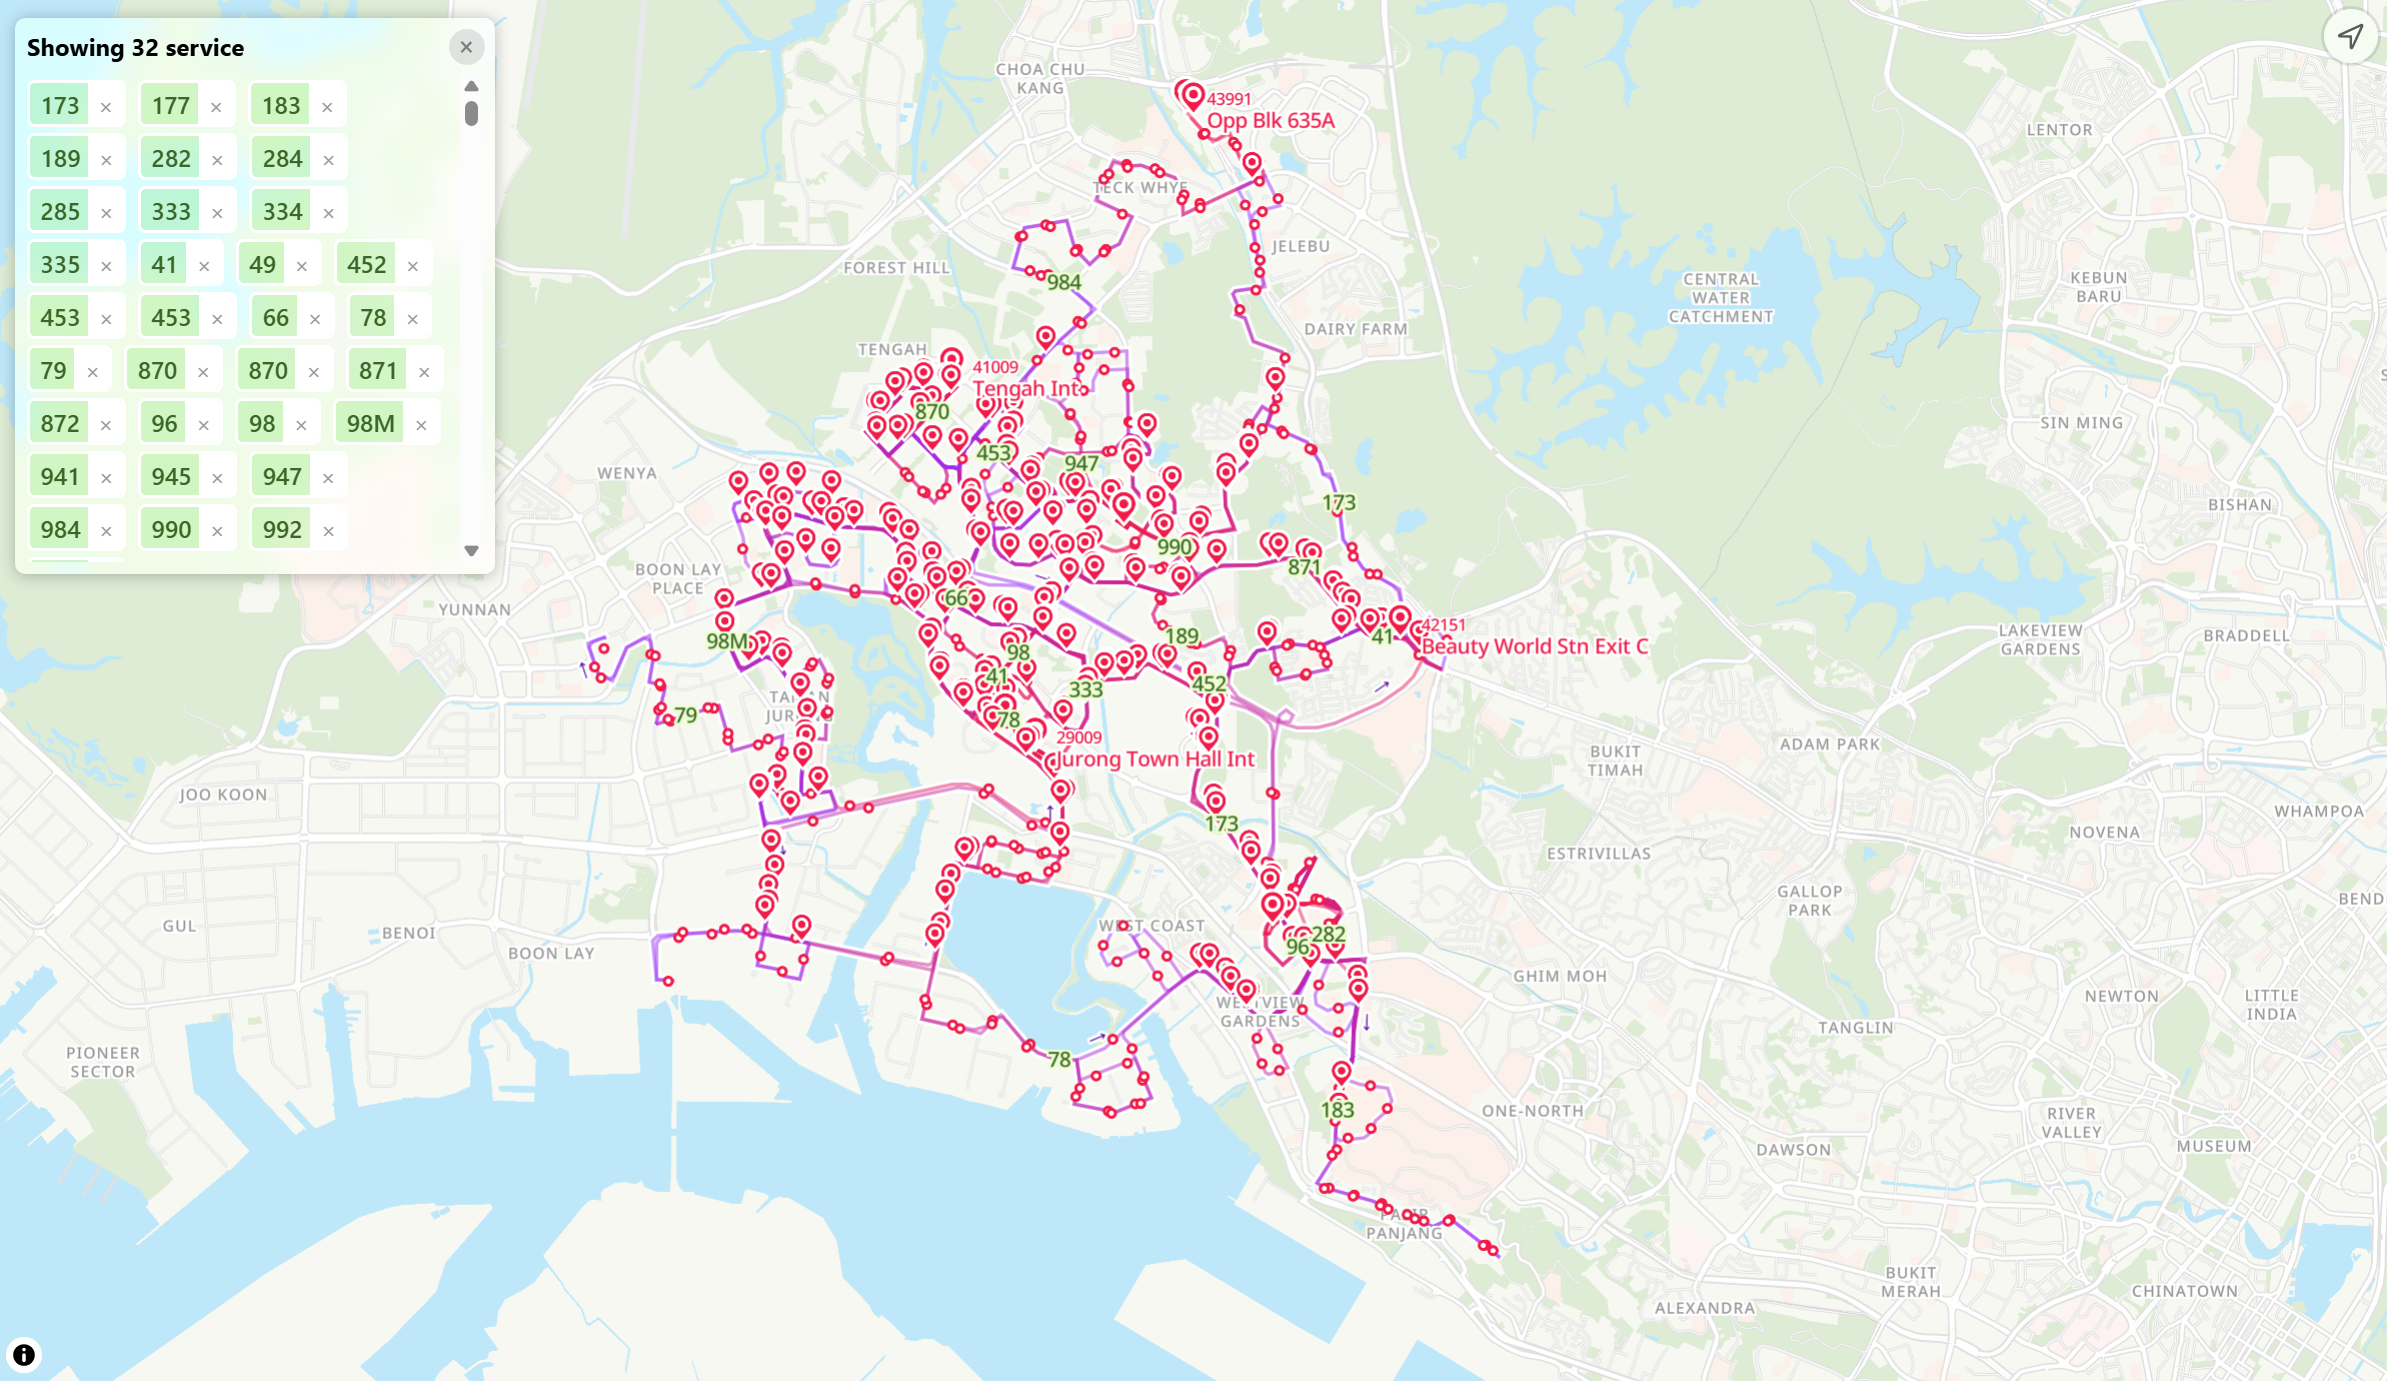
\includegraphics[width=0.88\linewidth]{figures/study_case.png}
    \caption{Spatial layout of the base Tower-derived network in the Jurong area.}
    \label{fig:case-study-map}
\end{figure}

% TODO: Check why the high-frequency scenario has fewer buses than the base scenario in the current generated data.
\begin{table}[htbp]
\centering
\small
\caption{Main instance families and experimental use}
\label{tab:instance-families}
\resizebox{\textwidth}{!}{%
\begin{tabular}{@{}lllll@{}}
\toprule
\textbf{Instance family} & \textbf{Data source or variant} & \textbf{Varied dimension} & \textbf{Primary use} & \textbf{Compared methods} \\
\midrule
\texttt{S-3}, \texttt{M-3}, \texttt{B-3}, \texttt{L-3} & \texttt{tower\_small}, \texttt{tower\_medium}, \texttt{tower}, \texttt{tower\_large} & Network scale, with three scenarios fixed & Network-scale ablation & Direct MILP, baseline integer L-shaped, lifted integer L-shaped, lifted two-phase, full method \\
\texttt{B-}k, $k\in\{3,5,10,20,40\}$ & \texttt{tower}, \texttt{tower\_5}, \texttt{tower\_10}, \texttt{tower\_20}, \texttt{tower\_40} & Scenario count, with base network fixed & Scenario-count scalability & Full method \\
\texttt{B-10-C}q, $q\in\{2,3,4,5,6\}$ & Capacity variants of \texttt{tower\_10} & Existing plug-in charger units, with base network and 10 scenarios fixed & Relaxation-gap stress test & Full method \\
\bottomrule
\multicolumn{5}{@{}l}{\footnotesize \texttt{B-3} is the representative base instance used for solution interpretation; larger $q$ indicates more existing plug-in charger units.} \\
\end{tabular}
}
\end{table}

\begin{table}[htbp]
\centering
\small
\caption{Parameter settings for the computational experiments}
\label{tab:parameter-settings}
\resizebox{\textwidth}{!}{%
\begin{tabular}{@{}>{\raggedright\arraybackslash}p{0.16\linewidth}>{\raggedright\arraybackslash}p{0.30\linewidth}>{\raggedright\arraybackslash}p{0.18\linewidth}>{\raggedright\arraybackslash}p{0.28\linewidth}@{}}
\toprule
\textbf{Parameter} & \textbf{Description} & \textbf{Value} & \textbf{Source} \\
\midrule
\multicolumn{4}{@{}l}{\textit{Battery and state of charge}} \\
$c^{\mathrm{bat}}$ & Daily-equivalent battery capacity cost & 0.148 USD/kWh/day & BloombergNEF price amortized over Wang et al. battery life \citep{bloombergnef_lithium-ion_2025,wang_reliable_2024} \\
$\mathcal{K}$ & Candidate route-level battery options & 10-kWh increments within instance bounds & Case-data preprocessing \\
$\underline{\rho},\overline{\rho}$ & Minimum and maximum state-of-charge fractions & 0.2, 0.8 & Wireless bus planning literature \citep{li_planning_2024} \\
\addlinespace
\multicolumn{4}{@{}l}{\textit{Charging operation}} \\
$\kappa$ & Maximum plug-in energy per occupied one-minute slot & 2.5 kWh/slot & \citet{najafi_integrated_2025} \\
$\bar q_v^{\mathrm{S}}$ & Visit-specific SWC opportunity limit & 1.0 kWh/min times eligible dwell time & \citet{wang_reliable_2024} \\
$\bar q_a^{\mathrm{D}}$ & Traversal-specific DWC opportunity limit & 1.0 kWh/min times traversal time & \citet{wang_reliable_2024} \\
$\eta^{\mathrm{P}}$ & Plug-in charging efficiency & 0.90 & \citet{li_planning_2024} \\
$\eta^{\mathrm{S}}$ & Stationary wireless charging efficiency & 0.85 & \citet{sun_optimizing_2024} \\
$\eta^{\mathrm{D}}$ & Dynamic wireless charging efficiency & 0.80 & \citet{sun_optimizing_2024} \\
$U_s$ & Existing plug-in charger units at plug-in location $s$ & 4 chargers in the base setting & Case-study assumption \\
\addlinespace
\multicolumn{4}{@{}l}{\textit{Infrastructure and electricity cost}} \\
$T^{\mathrm{fac}}$ & Facility amortization horizon & 30 years & \citet{wang_reliable_2024} \\
$c_s^{\mathrm{S}}$ & Daily-equivalent cost of an SWC facility & 2.16 USD/day & \citet{wang_reliable_2024} \\
$c_l^{\mathrm{D}}$ & Daily-equivalent cost of a DWC facility on link $l$ & 9 USD/km/day times link length, plus 0.90 USD/day & \citet{wang_reliable_2024} \\
$c^{\mathrm{day}}$ & Daytime electricity price & 0.1922 USD/kWh & Singapore tariff data \citep{singstat_electricity_2026} \\
$c^{\mathrm{night}}$ & Nighttime electricity price & 0.1233 USD/kWh & Singapore tariff data \citep{singstat_electricity_2026} \\
\bottomrule
\end{tabular}
}
\end{table}

\subsection{Solution characteristics on the base Tower instance}
\label{subsec:solution-characteristics}

This subsection will use the full-method solution for \texttt{B-3} to examine whether the optimized plan is interpretable at the facility, battery, and charging levels.
Table~\ref{tab:planned-solution-summary} lists the outputs to be reported once the final decision data are extracted.

\begin{table}[htbp]
\centering
\small
\caption{Planned summary of the representative \texttt{B-3} solution}
\label{tab:planned-solution-summary}
\begin{tabular}{@{}>{\raggedright\arraybackslash}p{0.22\linewidth}>{\raggedright\arraybackslash}p{0.36\linewidth}>{\raggedright\arraybackslash}p{0.34\linewidth}@{}}
\toprule
\textbf{Result block} & \textbf{Reported quantities} & \textbf{Purpose} \\
\midrule
Cost composition & Facility, expected battery, daytime charging, and overnight charging costs & Verify how the objective is distributed across planning and recourse decisions \\
Facility deployment & Numbers of selected SWC stations and DWC links, together with representative selected locations & Identify where the optimized layout creates charging opportunities \\
Battery adaptation & Route-level battery capacities by scenario and their minimum, median, and maximum values & Show how battery configurations adapt across service plans \\
Charging allocation & Plug-in, SWC, DWC, and overnight charging energy, plus peak plug-in utilization & Describe how wireless deployment and shared plug-in capacity interact \\
\bottomrule
\end{tabular}
\end{table}

A second compact table will list representative selected stations or links, their facility type, and the routes and scenarios that use them.
The accompanying analysis will distinguish shared network-level deployments from route-specific charging opportunities and will relate the selected battery capacities to residual plug-in charging demand.

% TODO: Populate both solution-characteristics tables after extracting the final B-3 decisions.

\subsection{Network-scale algorithmic ablation}
\label{subsec:network-scale-results}

The network-scale ablation fixes the number of service-plan scenarios at three and increases the physical network size from \texttt{S-3} to \texttt{L-3}.
Table~\ref{tab:network-ablation} reports the available runs across the core benchmark ladder and tracks how the solvable boundary changes as the lifted and two-phase components are introduced.

\begin{table}[htbp]
\centering
\small
\caption{Network-scale ablation under three service-plan scenarios}
\label{tab:network-ablation}
\resizebox{\textwidth}{!}{%
\begin{tabular}{@{}lccccc@{}}
\toprule
\textbf{Instance} & \textbf{Direct MILP} & \textbf{Baseline integer L-shaped} & \textbf{Lifted integer L-shaped} & \textbf{Lifted two-phase} & \textbf{Full method} \\
\midrule
\texttt{S-3} & Opt., 4.2s & TL, 98.37\% & TL, 77.84\% & Opt., 0.4s & Opt., 0.4s \\
\texttt{M-3} & TL, 0.27\% & n.r. & n.r. & Opt., 25.8s & Opt., 25.7s \\
\texttt{B-3} & n.r. & n.r. & n.r. & Opt., 29.4s & Opt., 32.2s \\
\texttt{L-3} & n.r. & n.r. & n.r. & TL, 0.092\% & TL, 0.092\% \\
\bottomrule
\multicolumn{6}{@{}l}{\footnotesize Opt. = reached the prescribed optimality tolerance; TL = 7200s time limit; n.r. = not reported in the current run set.} \\
\multicolumn{6}{@{}l}{\footnotesize Percentages are final relative gaps at termination.} \\
\end{tabular}
}
\end{table}

The results identify the two-phase structure as the main computational transition in this run set.
On \texttt{S-3}, the direct MILP is still easy, but the standard integer L-shaped variants make little progress within the time limit because their master lower bounds remain weak.
Once route-level lower bounding and exact Phase 2 verification are introduced, both two-phase variants solve \texttt{S-3}, \texttt{M-3}, and \texttt{B-3}.
Both two-phase variants reach the time limit on \texttt{L-3}; Table~\ref{tab:mechanism-contrast} reports their terminal bounds.

\begin{table}[htbp]
\centering
\small
\caption{Two-phase boundary diagnostics on the largest three-scenario instance}
\label{tab:mechanism-contrast}
\begin{tabular}{@{}lrrrrr@{}}
\toprule
\textbf{Method} & \textbf{Status} & \textbf{UB} & \textbf{LB} & \textbf{Gap (\%)} & \textbf{Time (s)} \\
\midrule
Lifted two-phase & TL & 27251.656 & 27226.537 & 0.092 & 7217.5 \\
Full method & TL & 27251.656 & 27226.537 & 0.092 & 7231.9 \\
\bottomrule
\multicolumn{6}{@{}l}{\footnotesize Both runs stop during Phase 2.} \\
\end{tabular}
\end{table}

The identical terminal bounds place the current network-scale boundary between \texttt{B-3} and \texttt{L-3} and show no additional benefit from the full-method enhancements on this instance.
Exact Phase 2 verification remains the limiting operation at this scale.

\subsection{Scenario-count scalability}
\label{subsec:scenario-scale-results}

This subsection uses the \texttt{B-}k family, with $k\in\{3,5,10,20,40\}$, to test scenario-count scalability on the base Tower-derived network.
To isolate growth in the scenario dimension while holding the network and algorithm fixed, Table~\ref{tab:scenario-scalability} reports the full method and separates Phase 1 and Phase 2 time.

\begin{table}[htbp]
\centering
\small
\caption{Scenario-count scalability on the base Tower-derived network}
\label{tab:scenario-scalability}
\resizebox{\textwidth}{!}{%
\begin{tabular}{@{}lrrrrrr@{}}
\toprule
\textbf{Instance} & \textbf{UB} & \textbf{LB} & \textbf{Gap (\%)} & \textbf{P1 time (s)} & \textbf{P2 time (s)} & \textbf{Total (s)} \\
\midrule
\texttt{B-3}  & 7869.832 & 7869.814 & 0.000 & 19.2 & 13.1 & 32.2 \\
\texttt{B-5}  & 7852.604 & 7852.340 & 0.003 & 27.4 & 30.3 & 57.7 \\
\texttt{B-10} & 7862.021 & 7861.809 & 0.003 & 59.0 & 60.6 & 119.7 \\
\texttt{B-20} & 7850.547 & 7850.375 & 0.002 & 126.6 & 120.8 & 247.4 \\
\texttt{B-40} & 7849.108 & 7848.937 & 0.002 & 345.5 & 580.9 & 926.4 \\
\bottomrule
\multicolumn{7}{@{}l}{\footnotesize All five runs converge within the prescribed tolerance; reported times are wall-clock seconds.} \\
\end{tabular}
}
\end{table}

The full method solves all tested scenario counts within the prescribed tolerance.
Total solution time increases from 32.2 seconds for \texttt{B-3} to 926.4 seconds for \texttt{B-40}, while all final gaps remain below 0.004\%.
Both phases grow with the scenario count, and Phase 2 becomes the larger time component at 40 scenarios because each master candidate requires more exact scenario evaluations.

\subsection{Capacity-coupling and relaxation-gap stress test}
\label{subsec:capacity-coupling-results}

This subsection uses \texttt{B-10-C2} through \texttt{B-10-C6} to test the effect of shared plug-in charger capacity on the relaxation-verification structure.
All five variants are built from \texttt{B-10}; only the number of existing plug-in chargers is varied.
Tighter capacity increases cross-route competition that is absent from the Phase 1 relaxation in Proposition~\ref{prop:phase-one-lb}, whereas looser capacity should bring the relaxed and exact recourse problems closer.
Table~\ref{tab:capacity-coupling} reports the full method only and uses the initial Phase 2 gap as a transition diagnostic for the complete algorithm.

\begin{table}[htbp]
\centering
\small
\caption{Capacity-coupling and relaxation-gap stress test on \texttt{B-10}}
\label{tab:capacity-coupling}
\resizebox{\textwidth}{!}{%
\begin{tabular}{@{}lrrrrrr@{}}
\toprule
\textbf{Instance} & \textbf{Status} & \textbf{UB} & \textbf{LB} & \textbf{Final gap (\%)} & \textbf{Initial P2 gap (\%)} & \textbf{Total (s)} \\
\midrule
\texttt{C2} & TL & -- & -- & -- & -- & 7243.1 \\
\texttt{C3} & Opt. & 7871.295 & 7870.696 & 0.008 & 0.676 & 280.5 \\
\texttt{C4} & Opt. & 7862.021 & 7861.809 & 0.003 & 0.562 & 148.2 \\
\texttt{C5} & Opt. & 7859.664 & 7859.497 & 0.002 & 0.532 & 95.9 \\
\texttt{C6} & Opt. & 7859.271 & 7859.164 & 0.001 & 0.527 & 114.0 \\
\bottomrule
\multicolumn{7}{@{}l}{\footnotesize \texttt{C}q denotes $q$ existing plug-in chargers at each plug-in charging location. \texttt{C2} reaches the Phase 2 time limit before a verified objective pair is recorded.} \\
\end{tabular}
}
\end{table}

As plug-in capacity increases from \texttt{C3} to \texttt{C6}, the initial Phase 2 gap falls from 0.676\% to 0.527\%, and the final optimality gaps after convergence remain below 0.008\%.
The tightest reported setting, \texttt{C2}, is qualitatively different: Phase 1 still solves the relaxed problem quickly, but Phase 2 repeatedly separates feasibility cuts and reaches the time limit.
Thus, the complete method handles the tested \texttt{C3}--\texttt{C6} range, while \texttt{C2} exposes a clear limitation: sufficiently tight shared capacity can make exact verification the computational bottleneck.

\section{Conclusion}
\label{sec:conclusion}

This paper studies a two-stage wireless charging facility-location problem for electric-bus systems under service-plan uncertainty.
The model treats SWC and DWC deployment as strategic here-and-now decisions, while route-level battery selection and representative-day charging operations adapt after each service-plan scenario is realized.
The resulting recourse structure captures how wireless charging opportunities affect battery requirements and residual demand for limited shared plug-in fast chargers.

The main methodological contribution is an exact decomposition framework for this shared-resource mixed-integer recourse structure.
The method uses an exact lifted reformulation that keeps scenario-dependent battery choices adaptive, a nested scenario--route relaxation--verification decomposition, and joint-resource direction-selective monotonicity cuts.
Phase 1 route-level LP relaxations obtain valid lower bounds and cuts, Phase 2 restores exact mixed-integer operational verification, and the strengthened full method applies monotonicity cuts where they are valid for exact recourse.
Under exact master and recourse separation, the complete procedure converges to an optimal solution of the original two-stage formulation.

The computational study is designed to show how each algorithmic component contributes to scalability.
The base planning instance illustrates the type of wireless facility layout and adaptive battery decisions produced by the model.
The ablation, scenario-scaling, and capacity-coupling experiments then evaluate when the direct solver and simpler decomposition variants become insufficient and when the full method remains effective.

Several limitations define natural extensions.
The current experiments use constructed service-plan scenarios, treat plug-in fast-charging infrastructure as exogenous, and do not endogenize the feedback from battery weight to route-level energy consumption.
Future work can develop richer scenario-generation models, jointly optimize wireless and plug-in charging expansion, incorporate operational uncertainty, and apply the lifted two-phase decomposition idea to other stochastic infrastructure-planning problems with shared-resource recourse.


\appendix
\section{Model Notation}
\label{app:model-details}

\begin{table}[htbp]
\centering
\scriptsize
\setlength{\tabcolsep}{3pt}
\renewcommand{\arraystretch}{0.94}
\caption{Summary of notation}
\label{tab:notation}
\begin{tabular}{@{}>{\raggedright\arraybackslash}p{0.23\linewidth}>{\raggedright\arraybackslash}p{0.71\linewidth}@{}}
\toprule
\textbf{Symbol} & \textbf{Description} \\
\midrule
\multicolumn{2}{@{}l}{\textit{Sets and indices}} \\
$\Omega$ & Set of service-plan scenarios, indexed by $\omega$ \\
$\mathcal{S}$ & Set of stations, indexed by $s$ \\
$\mathcal{L}$ & Set of directed links between consecutive stations, indexed by $l$ \\
$\mathcal{C}$ & Set of existing interchanges or hubs equipped with plug-in chargers, $\mathcal{C}\subseteq\mathcal{S}$ \\
$\mathcal{R}$ & Set of routes, indexed by $r$ \\
$\mathcal{K}$ & Set of candidate battery-capacity options, indexed by $k$ \\
$\mathcal{M}_{\omega,r}$ & Set of bus trip chains on route $r$ under scenario $\omega$, indexed by $m$ \\
$\mathcal{V}_{\omega,r}$ & Set of station visits on route $r$ under scenario $\omega$, indexed by $v$ \\
$\mathcal{V}^{\mathrm{P}}_{\omega,r}$ & Set of plug-in charging visits on route $r$ under scenario $\omega$ \\
$\mathcal{V}^{\mathrm{S}}_{\omega,r}$ & Set of SWC-eligible station visits on route $r$ under scenario $\omega$ \\
$\mathcal{A}_{\omega,r}$ & Set of directed link traversals on route $r$ under scenario $\omega$, indexed by $a$ \\
$\mathcal{T}_\omega$ & Relevant plug-in charging time periods under scenario $\omega$ \\
$\mathcal{T}_v$ & Time periods during which plug-in charging visit $v$ can occupy a plug-in charger \\
\addlinespace
\multicolumn{2}{@{}l}{\textit{Parameters}} \\
$p_\omega$ & Probability of scenario $\omega$ \\
$c_s^{\mathrm{S}}$ & Representative-day equivalent cost of installing SWC at station $s$ \\
$c_l^{\mathrm{D}}$ & Representative-day equivalent cost of installing DWC on link $l$ \\
$c^{\mathrm{bat}}$ & Representative-day equivalent battery capacity cost per kWh \\
$c^{\mathrm{day}},c^{\mathrm{night}}$ & Daytime and overnight electricity prices \\
$n_{\omega,r}$ & Fleet-size requirement for route $r$ under scenario $\omega$ \\
$\beta_k$ & Battery capacity value represented by option $k$ \\
$d_a$ & Energy consumption associated with directed link traversal $a$ \\
$d_m^{0}$ & Boundary energy consumption from the depot to the first station visit of trip chain $m$ \\
$d_m^{N}$ & Boundary energy consumption from the terminal station visit of trip chain $m$ back to the depot \\
$U_s$ & Number of existing plug-in chargers at station $s$ \\
$\kappa$ & Grid-side energy delivered by one occupied plug-in time slot \\
$\bar{q}^{\mathrm{S}}_v$ & Maximum SWC energy available during station visit $v$ \\
$\bar{q}^{\mathrm{D}}_a$ & Maximum DWC energy available during directed link traversal $a$ \\
$\eta^{\mathrm{P}},\eta^{\mathrm{S}},\eta^{\mathrm{D}}$ & Charging efficiencies for plug-in charging, SWC, and DWC \\
$\underline{\rho},\overline{\rho}$ & Minimum and maximum state-of-charge fractions \\
\addlinespace
\multicolumn{2}{@{}l}{\textit{Derived quantities and functions}} \\
$s(v)$ & Physical station associated with station visit $v$ \\
$\ell(a)$ & Directed link associated with traversal $a$ \\
$\mathrm{tail}(a)$ & Departure station visit of traversal $a$ \\
$\mathrm{head}(a)$ & Arrival station visit of traversal $a$ \\
$v_m^{0}$ & First station visit of trip chain $m$ \\
$v_m^{N}$ & Terminal station visit of trip chain $m$ \\
\addlinespace
\multicolumn{2}{@{}l}{\textit{Decision variables}} \\
$w_s^{\mathrm{S}}$ & 1 if SWC is installed at station $s\in\mathcal{S}\setminus\mathcal{C}$, 0 otherwise \\
$w_l^{\mathrm{D}}$ & 1 if DWC is installed on link $l\in\mathcal{L}$, 0 otherwise \\
$z_{\omega,r,k}$ & 1 if route $r$ uses battery capacity option $k$ in scenario $\omega$, 0 otherwise \\
$B_{\omega,r}$ & Selected battery capacity for route $r$ in scenario $\omega$ \\
$y_\omega$ & Vector of scenario-level charging, plug-in occupancy, and energy-state decisions in scenario $\omega$ \\
$q_v^{\mathrm{P}}$ & Plug-in charging energy assigned during plug-in visit $v$ \\
$q^{\mathrm{S}}_v$ & SWC energy assigned during SWC-eligible station visit $v$ \\
$q^{\mathrm{D}}_a$ & DWC energy assigned to directed link traversal $a$ \\
$q_m^{\mathrm{N}}$ & Overnight charging energy assigned after trip chain $m$ returns to the depot \\
$e^{\mathrm{arr}}_v,e^{\mathrm{dep}}_v$ & Battery energy state at arrival and departure of station visit $v$ \\
$x_{v\tau}$ & 1 if plug-in charging visit $v$ occupies one plug-in charger at time $\tau$, 0 otherwise \\
\bottomrule
\end{tabular}
\end{table}

\section{Proofs}
\label{app:proofs}

% TODO: Move long proof details here once the main propositions are stable.

\FloatBarrier
\section{Additional Computational Results}
\label{app:extra-results}

\subsection{Computational parameter settings}
\label{app:computational-parameters}

Facility and battery capital costs are annualized and converted to representative-day equivalents to be comparable with daily charging costs.
Table~\ref{tab:parameter-settings} summarizes the common physical and economic parameters.

\begin{table}[!htbp]
\centering
\small
\caption{Parameter settings for the computational experiments}
\label{tab:parameter-settings}
\begin{tabular}{@{}>{\raggedright\arraybackslash}p{0.26\linewidth}>{\raggedright\arraybackslash}p{0.37\linewidth}>{\raggedright\arraybackslash}p{0.29\linewidth}@{}}
\toprule
\textbf{Parameter} & \textbf{Value} & \textbf{Source} \\
\midrule
\multicolumn{3}{@{}l}{\textit{Battery and state of charge}} \\
Battery capacity cost $c^{\mathrm{bat}}$ & 0.148 USD/kWh/day & \citet{bloombergnef_lithium-ion_2025}; \citet{wang_reliable_2024} \\
State-of-charge bounds $(\underline{\rho},\overline{\rho})$ & $(0.2,0.8)$ & \citet{li_planning_2024} \\
\addlinespace
\multicolumn{3}{@{}l}{\textit{Charging operation}} \\
Plug-in energy rate $\kappa$ & 2.5 kWh per one-minute slot & \citet{najafi_integrated_2025} \\
SWC opportunity limit $\bar q_v^{\mathrm S}$ & 1.0 kWh/min times eligible dwell time & \citet{wang_reliable_2024} \\
DWC opportunity limit $\bar q_a^{\mathrm D}$ & 1.0 kWh/min times traversal time & \citet{wang_reliable_2024} \\
Charging efficiencies $(\eta^{\mathrm P},\eta^{\mathrm S},\eta^{\mathrm D})$ & $(0.90,0.85,0.80)$ & \citet{li_planning_2024,sun_optimizing_2024} \\
\addlinespace
\multicolumn{3}{@{}l}{\textit{Infrastructure and electricity cost}} \\
Facility amortization horizon $T^{\mathrm{fac}}$ & 30 years & \citet{wang_reliable_2024} \\
SWC facility cost $c_s^{\mathrm S}$ & 2.16 USD/day & \citet{wang_reliable_2024} \\
DWC facility cost $c_l^{\mathrm D}$ & 9 USD/km/day times link length, plus 0.90 USD/day & \citet{wang_reliable_2024} \\
Electricity prices $(c^{\mathrm{day}},c^{\mathrm{night}})$ & $(0.1922,0.1233)$ USD/kWh & \citet{singstat_electricity_2026} \\
\bottomrule
\end{tabular}
\end{table}

% TODO: Add supplementary logs, tables, or robustness checks if needed.


\FloatBarrier
\bibliographystyle{elsarticle-harv}
\bibliography{refs}

\end{document}
